%% LyX 2.0.2 created this file.  For more info, see http://www.lyx.org/. 
%% Do not edit unless you really know what you are doing. 
\documentclass[english,noae]{article} 
\usepackage[T1]{fontenc} 
\usepackage{amsmath} 
\usepackage{amssymb} 

\makeatletter 

%%%%%%%%%%%%%%%%%%%%%%%%%%%%%% LyX specific LaTeX commands. 
%% Because html converters don't know tabularnewline 
\providecommand{\tabularnewline}{\\} 

%%%%%%%%%%%%%%%%%%%%%%%%%%%%%% Textclass specific LaTeX commands. 

\makeatother 

\usepackage{babel} 
\usepackage{Sweave} 

\newtheorem{thm}{\protect\theoremname}
\theoremstyle{definition}
\newtheorem{defn}[thm]{\protect\definitionname}
\theoremstyle{plain}
\newtheorem{prop}[thm]{\protect\propositionname}
\newtheorem{definition}{Definition}[chapter]
\newtheorem{proposition}{Proposition}[chapter]

\begin{document} 
\Sconcordance{concordance:dizzysNewInfec.tex:dizzysNewInfec.Rnw:%
1 167 1 1 2 1 0 1 5 4 0 1 3 5 0 1 2 1 1 1 2 1 0 1 1 4 0 1 2 6 1 1 3 2 0 %
1 1 4 0 1 2 1 1 1 2 1 0 1 1 4 0 1 2 1 1 1 2 1 0 1 1 4 0 1 2 3 1 1 2 1 0 %
1 1 4 0 1 2 1 1 1 5 4 0 1 1 1 4 2 0 1 1 4 0 1 2 16 1}

\Sconcordance{concordance:dizzysNewInfec.tex:dizzysNewInfec.Rnw:%
1 167 1 1 2 1 0 1 5 4 0 1 3 5 0 1 2 1 1 1 2 1 0 1 1 4 0 1 2 6 1 1 3 2 0 %
1 1 4 0 1 2 1 1 1 2 1 0 1 1 4 0 1 2 1 1 1 2 1 0 1 1 4 0 1 2 3 1 1 2 1 0 %
1 1 4 0 1 2 1 1 1 5 4 0 1 1 1 4 2 0 1 1 4 0 1 2 16 1}
 

\title{$\mathbf{dizzys}$: Efficient deterministic/stochastic simulations 
for metapopulation SIR/SEIR models of epidemics by integrating C++ into R} 


\author{TRAN Thi Cam Giang} 
\maketitle 
\begin{abstract} 
Stochastic and analytical methods are widely applied for the analysis of epidemic models. Many simulation softwares as well as packages are proposed to help scientists observe fluctuations of infectious diseases over time. These tools simulate epidemic models either by dealing with a set of ordinary differential equations (ODEs) or by applying the stochastic simulation algorithm (SSA) of Gillespie. Simple epidemic models work well on these software tools. However, the accuracy, the simulation speed, and the complexity of models that the tools can simulate are three main drawbacks that always prompt us not to stop improving tools to increase efficient implementations available in software tools. Moreover, rather than dynamics of infectious diseases, predicting the potential spread of an infectious disease in a meta-population is the most difficult problem for scientists. To give an exact prediction about propagation of infectious diseases in a meta-population, we need to make simulations in a complex meta-population with many interconnected sub-populations where the meta-population takes into account many factors about the pathogen, the climatic conditions and simultaneously the interactions between sub-populations. Therefore, we introduce the "dizzysNewInfec" package that allows us to exactly simulate and accurately analyze dynamics of an infectious disease in a meta-population of interconnected sub-populations by using two basic and common disease models SIR and SEIR, and by implementing the direct algorithm of Gillespie in 1977 and the adaptive tau leaping to approximate the trajectory of a continuous-time stochastic process. In addition, on the technical aspect, this package integrates C++ in R, we use C++ to build algorithms, and use R to show two-dimensional and three-dimensional interfaces and use the available statistic functions in R to analyze obtained results. Hence, dizzysNewInfec, it speeds up simulations, it is very easy to install, to use and to show trajectories of disease evolution over time in a meta-population of sub-populations.
\end{abstract} 

\section*{Introduction} 
Fundamentally, Kermack-McKendrick gave the first epidemic model to provide a mathematical description of the kinetic transmission of an infectious disease in an unstructured sub-population. Due to this model, today we have known well the SIR and SEIR deterministic epidemic models. These two basic epidemic models are very popularly used by scientists. The reactions in the system are modelled by a set of Ordinary Differential Equations (ODEs) [li2007stochastic]. The deterministic method is the simplest to solve an epidemic model. The main idea of this method is to solve a single differential equation per species of the model. Basically, the deterministic method uses the law of mass action that has applicability in many areas of science. In chemistry, it is also called Fundamental Law of Chemical Kinetics (the study of rates of chemical reactions), introduced   by the Norwegian scientists Cato M. Guldberg in 1864-1879 and Peter Waage. The law of mass action shows a simple relation between reaction rate and molecular component concentrations. For a set of initial molecular concentrations given, the law of mass action permits us to see the component concentrations over time. The states of a reaction are a homogeneous, free medium. The reaction rate will be directly scaled with the concentrations of the elements. Most systems can use the traditional deterministic approaches to simulate. It is evident that many systems such as some biochemical systems consist of random, discrete interactions between individual elements. In fact, we have applied the deterministic model in the epidemiology to solve epidemic models such as the SEIR and SIR models. However, in the case, these systems become smaller and smaller, the traditional deterministic models may not be accurate. In addition, in the deterministic approach, the time evolution of a reacting system is assumed that it is both continuous and deterministic. But in fact, molecular population levels can change only by discrete integer amounts. It is the reason for that this time evolution is not both a continuous process and a discrete process. Hence, the deterministic approach is impossible to predict the exact molecular population levels at some future times unless we can compute exactly the precise positions and velocities of all molecules in the system. It is the reason for that the fluctuations of these systems can be simulated exactly by applying stochastic models via Stochastic Simulation Algorithms (SSA) [gillespie1976general,gillespie1977exact]. The SSA uses Monte Carlo (MC) methods to study the time evolution of the jump process. Because the basis feature of the Monte Carlo simulation is insensitive to the dimensionality of the problem, and the work grows linearly with the number of reaction channels in the model. The SSA describes time-evolution statistically correct trajectories of finite populations in continuous time by solving the corresponding stochastic differential equations. Using the stochastic models can solve three questions. (1) These models take account the discrete character of the number of elements and the evidently random character of collision among elements. (2) They coincide with the theories of the dynamic and stochastic processes. (3) They are a good idea to describe "small systems" and "unstable systems". The main idea of the stochastic models is that element reactions are essentially random processes. We don't know certainly how a reaction occurs at a moment. We also call it the process stochasticity. Demographic stochasticity is considered as fluctuation in population processes that is based the random nature of events at the level of the individual. Each event is related to one baseline probability fixed, individuals are presented in differing fates due to chance. In addition to the demographic stochasticity, the number of infectious, susceptible, exposed and recovered individuals in a meta-population infected by an infectious disease is now required to be an integer. Modeling approaches that incorporate demographic stochasticity are called event-driven methods. These methods require explicit consideration of events. The first approach published by Daniel T.Gillespie in 1976 {gillespie1976general} is an exact stochastic simulation approach for chemical kinetics. The Gillespie stochastic simulation algorithm (SSA) has become the standard procedure of the discrete-event modelling by taking proper value of the available randomness in such a system. The methods modelling the event-driven model demands explicit presentation of events. Therefore, the "dizzysNewInfec" package permits us to obtain the dynamics of the deterministic and the stochastic dynamics of two basic epidemic models SIR and SEIR.  We use the exact algorithm of Gillespie in 1977 and the "adaptive tau-leaping” algorithm in the package. With these two algorithms, each has its private advantages and its private disadvantages. For the exact algorithm, it gives us a really exact 
approach of simulating population-based time-to-event through two steps with many iterations of 1) searching the time of next event by an exponentially distributed function and 2) searching the nature of next event. Each single event in the Gillespie's solution is explicitly simulated, so this exact simulation becomes exceedingly slow and impractical in systems where the transition rate grows large over time. Hence, approximate models are born instead of the Gillespie's solution, they are concerned with larger transition rates and with increasing simulation speed while still maintaining reasonable accuracy. The "adaptive tau-leaping" algorithm known as an approximate method reduces the number of iterations by treating transition rates as constant over time periods 
for which this approximation leads to little error [Cao2007]. 

The SEIR epidemic model used in our package have successful described hosts within a population as Susceptible (the number of individuals not yet infected with the disease), Exposed (the number of individuals who are infected with the disease but not infectious), Infected (the number of individuals who have been infected with the disease and are capable of spreading the disease), and Recovered (the number of individuals who have successfully cleared the infection). We ignore population demography-births, deaths, and migration. So we have only three transitions: 
\begin{equation}
S \rightarrow E,  E \rightarrow I,  I \rightarrow R.  
\end{equation}
It is obvious that the second and third of these transitions are easier, so we focus on the first transition in which the level of the infectious disease influences strongly the disease transmission rate from a susceptible individual into the infected class. If this first step doesn't occur, all infected individuals can go to the recovered class. This first transition plays an important role in studying fluctuation of disease. Many researches have been tried to find the "infectious period" (the amount of time spent in the infectious class). They have found that for acute infections, the "infectious period" is distributed around some mean values that we can estimate from clinical data. To present enough properties of the "infectious period" by formulations, we have to depend upon three main factors of the disease transmission from S to E : the prevalence of infecteds, the underlying population contact structure, and the probability of transmission given contact. For a directly transmitted disease, the key factor is the contact between susceptible and infected individuals. Hence, in this package "dizzysNewInfe", we interpret the "infectious period" in more detailed, and realistic contexts. We introduce a new formula of the probabilistic derivation of multipopulation epidemic model called NIIF. We study the case where agent $x$ native from subpopulation $i$ visits sub-population $j$. In a meta-population of sub-populations, during a small interval of time $\delta t$, each native individual of the sub-population $i$ visits one single sub-population $j$ (with probability $\rho_{ij}$) and will see on average $K_{j}$. These individuals come from all sub-populations. This is absolutely a new interpretation about the infection between individuals and the propagation of disease between sub-population. In previous research described in [keeling2011], the authors always assumed that both the number of people we meet and the number of infected people we meet are fixed. This assumption simplifies the relations between individuals and between sub-populations. It's the reason for that the formula of the infection force did not present clearly the complex connections between individuals and between sub-populations in a meta-population. In our interpretation, we assume that for each sub-population $k$, the number of people native from $k$ that we meet during $\delta t$ follows a Poisson process. So both the number of people we meet and the number of infected people we meet during $\delta t$ should be random variables. 

In short, the \textbf{dizzysNewInfec} package implements both the exact solution and the approximate solution for the SIR and SEIR models. The package installs well the new interpretation of the infection force NIIF for SIR and SEIR meta-population models by integrating the R package and the C++ implementation. We can choose one of these two solutions to simulate when the number of sub-populations in a meta-population increases. Using C++ to perform the algorithms, and R to create interfaces makes the \textbf{dizzysNewInfec} package much faster and much easy to use than any pure R package.

\section*{Methods} 

In this section, first we will talk about the deterministic and stochastic SEIR models. Then, we will present transformation the SEIR model into the SIR model through the usage of the two algorithms. We hope that the models and the algorithms should be well understood before obtaining simulation results. 

\subsection*{Deterministic SEIR model:} 

To describe infectious diseases in a in a spatial context, we consider a meta-population of n sub-populations. In sub-population $i$ of size $N_{i}$, disease dynamics can be deterministically described by the following set of differential equations: 

\begin{eqnarray} 
\frac{dS_{i}}{dt} & = & \mu N_{i}-\lambda_{i}S_{i}-\mu S_{i}\label{eq:dS-1}\\ 
\frac{dE_{i}}{dt} & = & \lambda_{i}S_{i}-\mu E_{i}-\sigma E_{i}\\ 
\frac{dI_{i}}{dt} & = & \sigma E_{i}-\mu I_{i}-\gamma I_{i}\label{eq:infectieux-1}\\ 
\frac{dR_{i}}{dt} & = & \gamma I_{i}-\mu R_{i}\label{eq:dR-1} 
\end{eqnarray} 

where $S_{i}$, $E_{i}$, $I_{i}$ et $R_{i}$ are respectively the numbers of susceptible, exposed, infectious and recovered in this sub-population $i$. Individuals are born susceptible and die at a 
rate $\mu$, become infected with the force of infection $\lambda_{i}$, infectious after a latency period of an average duration of $1/\sigma$ and recover at the rate $\gamma$. In case the infectious contact rate is constant, the equilibrium values of the variables $S$, $E$, $I$ and $R$ can be expressed analytically (see appendix). The force of infection depends not only on the total population size $N_{i}$ and the number of infected $I_{i}$ in subpopulation $i$, but also in other sub-populations : 

\[
\lambda_{i}=\sum_{j}\rho_{ij}\kappa_{j}\log\left[1-\sum_{k=1}^{M}\left(\frac{\left|I_{k,t}\right|}{N_{k}}\times c_{ik}\times\xi_{jk}\right)\right]
\]

where 
$\rho_{i,j}$ the probability that an individual from sub-population $i$ visits sub-population $j$. 
$\kappa_{j}$ is the average number of contacts per unit of time a susceptible will have when visiting city. 
$c_{i,k}$ is the probability that a susceptible individual native from $i$ being in contact with another infected individual native from $k$. 
$\xi_{jk}$ refers to the probability that an individual $y$ meeting $x$ in  $C_{j}$ comes from  $C_{k}$. 
See appendix for detail on the construction of this equation. We can verify that in the limit case on one single subpopulation in the metapopulation ($i=j$ and $n=1$), we have :

\begin{equation}
\lambda_{i}=-\kappa_{i}\log(1-\frac{I_{i}}{N_{i}}\times c_{ii})
\end{equation}

In the case, we consider that the contact number $K_{i}$ is seasonally forced [Altizer2006]: 
\begin{equation} 
K_{i}(t)=K_{i0}\left[1+K_{i1}\cos\left(\frac{2\pi t}{T}+\varphi_{i}\right)\right]\label{eq:beta_i-1} 
\end{equation} 
where $K_{i0}$ and $K_{i1}$ are the mean value and amplitude of the contact number and $T$ and $\varphi_{i}$ are the period and the phase of the forcing. 
 
\subsection*{Stochastic models:} 
The stochastic model is built by depending upon the deterministic model. More detailed, this stochastic model relies on chance variation in risks of exposure, disease, and other factors. It is referred as an individual-level modeling, because every individual plays an important role in the model, so this stochastic model can consider well most small population size that the deterministic model can not do. To implement this SEIR stochastic model, there are many different methods. The first method "First Reaction Method" is born in 1976 by Gillespie. Then, according to this first method and these two key factors of demographic stochasticity models (event, randomness), many scientists have improved the first method, and created many better algorithms for stochastic simulations. There are two main types of methods, exact methods and approximative methods. The typical approach in exact methods most practitioners use, is the algorithm "Direct Method" of Gillespie(1977) improved from the first approach "First Reaction Method", and in approximative methods, is the "tau-leaping" method.
For the Direct Method (Gillespie 1977), the first step estimates the time until the next event, by accumulating the rates of all possible events. Then, by transforming event rates into probabilities, the method randomly selects one of these events. The time and numbers in each class are then updated according to which event is chosen. We repeat this process to iterate model through time. 
For the "tau-leaping" method, the main crux is the use of Poisson random variables to approximate the number of occurrences of each type of reaction event during a carefully selected time period, $\tau$ .
According to these two types of algorithms, the common point is both methods use continuous-time Markov process for which the transition rates are constants, isn't a function of time. The future state of the process, is only conditional on the present state, but independent of the past. However, for the exact algorithm, its advantage give us a really exact approach to simulate time-to-event model. This process is repeated to iterate the mode. GibsonBruck(2000) [KeelingRohani2008] modified the first reaction method and created the Next Reaction method that substantially more challenging to program but is significantly faster than even the method when there are a large number of different event types. The Direct, First Reaction and Next Reaction methods are all exact stochastic approaches of the underlying ordinary differential equations. But, its disadvantages are 1) noise in exact simulations only affects the probabilities associated with fates of individuals and the updating of each consecutive event is independent – there is no assumption concerning environmental stochasticity; 2) these exact solutions become too slow and impractical when any one transition rate is large, when there is a big number of sub-populations or one a big number of event in a meta-population. It is the reason for that, approximate models have been proposed instead of the exact stochastic methods. Gillespie (2001) has proposed a new method that decreases the simulation accuracy, but increases simulation speed. This is the "tau-leap method" known as an approximate method reduces the number of iterations by treating transition rates as constant over time periods for which this approximation leads to little error [KeelingRohani2008] as mentioned above. However, when we use the "tau-leap method", there is a possibility, the number of individual in each class can become negative.
According to Keeling2008 [KeelingRohani2008], the authors compared these methods together, they pointed out that when the population size increases, the simulation time of the three methods (First Reaction, Direct Method, tau -leap ) is almost augmented. The simulation time of the method "First Method" is maximum, it means that this is the slowest method, but the simulation time of the method "tau-leap" is minimum or the fastest. In the shape of my package, we use the direct method to exactly estimate spread of diseases in meta-population. Because the direct method is one exact approach and its simulation time isn't too slow and too fast. We use the approximate method to speed up simulations in the case where there are many sub-populations in a meta-population.


\subsubsection*{Direct method}

Based on the differential equations above, we give a stochastic version of this model. We use for that a population-based time-to-next-event model based on Gillespie's algorithm [Daniel.T.Gillespie1977]. Table \ref{tab:stoch_ev} lists all the events of the model, occurring 
in subpopulation $i$. 

\begin{table}[htpb] 
\begin{centering} 
\caption{\label{tab:stoch_ev}Events of the stochastic version of the model of equations, occuring in subpopulation $i$.} 

\par\end{centering} 

\centering{}\textbf{}% 
\begin{tabular}{lcc} 
\textbf{Events } & \textbf{Rates } & \textbf{Transitions }\tabularnewline 
\textbf{birth}  & $\mu N_{i}$  & $S_{i}\leftarrow S_{i}+1$ and $N_{i}\leftarrow N_{i}+1$ \tabularnewline 
\textbf{death of a susceptible } & \textbf{$\mu S_{i}$ } & \textbf{$S_{i}\leftarrow S_{i}-1$ }\tabularnewline 
\textbf{death of an exposed } & \textbf{$\mu E_{i}$ } & \textbf{$E_{i}\leftarrow E_{i}-1$ }\tabularnewline 
\textbf{death of an infected } & \textbf{$\mu I_{i}$ } & \textbf{$I_{i}\leftarrow I_{i}-1$ }\tabularnewline 
\textbf{death of an immune } & \textbf{$\mu R_{i}$ } & \textbf{$I_{i}\leftarrow I_{i}-1$ }\tabularnewline 
\textbf{infection } & \textbf{$\lambda_{i}S_{i}$ } & \textbf{$S_{i}\leftarrow S_{i}-1$ }and\textbf{ $E_{i}\leftarrow E_{i}+1$ }\tabularnewline 
\textbf{becoming infectious } & \textbf{$\sigma E_{i}$ } & \textbf{$E_{i}\leftarrow E_{i}-1$ }and\textbf{ $I_{i}\leftarrow I_{i}+1$ }\tabularnewline 
\textbf{recovery } & \textbf{$\gamma I_{i}$ } & \textbf{$I_{i}\leftarrow I_{i}-1$ }and\textbf{ $R_{i}\leftarrow R_{i}+1$ }\tabularnewline 
 &  & \tabularnewline 
\end{tabular} 
\end{table} 


To apply the Direct Method in a meta-population of n sub-populations, we know that at a moment $t$, there are only one single event fired in one single sub-population during one time unit $tstep$. Hence, we improve the Direct Method for one single population by adding a random number to calculate chance which sub-population to fire. Starting from the initial states, the stochastic simulation algorithms simulate the trajectory in population processes by repeatedly answering the following three big questions and updating the states. 

\begin{itemize}
\item When (time) will the next event occur?
\item Which subpopulation where the event will occur next?
\item Which event in the subpopulation will occur next?
\end{itemize}

Although, it is a small improvement in the original Direct Method, however it turns back much more benefits for a meta-population, it well presents the interactions between subpopulations in the metapopulation. 


\subsubsection*{Adaptive tau-leaping algorithm} 
In this step, we provide basic concepts for the adaptive tau-leaping algorithm by using the detailed description of Cao [Cao2007]. 

For the Markov process at time t, to describe a metapopulation of n subpopulations, we have: 

\textbf{state set:} X(t) 

$X(t):=[S_{1}(t),...,S_{n}(t),E_{1}(t),...,E_{n}(t),I_{1}(t),...,I_{n}(t),R_{1}(t),...,R_{n}(t)]$ 

each variables of $X(t)$ is defined on the non-negative integers. 

\textbf{set of allowable transitions:} ${\triangle_{j}}$, for each 
allowable transition, $j$, we define a rate $\lambda_{j}$, by using 
a function independent on t but dependent on the current state $X(t)$, 
to calculate transition rates given the state $(\lambda(X))$ through 
the deterministic model, and a vector of $n$ integers, $\triangle_{j}:=[\triangle_{j,1},...,\triangle_{j,n}]$, 
that reflects the change in state if this transition were followed: 
$X(t)+\triangle_{j}$. 

\textbf{time process: }modeling on a time-homogeneous process. 

\textbf{operation:} with the SEIR model, the package simulates a trajectory from time $0$ to a stopping time $tmax$. Based on the description of Cao and al. in 2007, a good time period of length $\tau$ is during which all transition rates remain approximately constant and all $n$ state variables remain greater than zero with probability$\thicksim1$. Then, by using the Poisson-dustributed number of transitions, that should have occurred during this period: $X(t+\tau)\approx X(t)+\sum_{j}y_{j}\triangle_{j}$ where $y_{j}\thicksim Poisson(\tau\lambda_{j})$. To successfully 
apply this algorithm, we need to know that, transition rates frequently change and in balancing efficiency with accuracy when selecting these time periods to leap over. 

In short, in the package "dizzysNewInfec" we have build successfully the Direct method and "tau-leap method" for a meta-population. In the particular case, there is one single sub-population, the Direct Method and "tau-leap" method for a meta-population are similar to the original methods.


\subsection*{Transformation SEIR model into SIR model:} 

The SIR model used in this package is the SIR model with births and death. By observing this SEIR model, if we give a numerical value for the parameter $\sigma$ then a SEIR model would have. On the other side, if we give $Inf$ (to infinity) the parameter $\sigma$ then we have a SIR model with birth and death (because, basically, a SEIR model tends to a SIR model when $\sigma$ tends to infinity). 

\section*{Example 1}
The deterministic SEIR model with one subpopulation by exploiting the 'seir' function in the package.

\begin{Schunk}
\begin{Sinput}
> library(dizzysNewInfec)
> # We have the values of parameters and of variables. 
> # Here, we have S=E=I=R=NULL and N=1e7.
> # It means that we use N=1e7 to calculate the equilibrium values of variables.
> obj<- globSEIRNewInfec(typeSIMU="deterministic",duration=10*365,mu=1/(70*365),sigma=1/8,gamma=1/5,
+ phiPHASE=0,nbCONTACT0=100,nbCONTACT1=0.1,nbVilles=1,S=NULL,E=NULL,I=NULL,R=NULL,N=1e7)
> # Use the plot function of the seir class
> plot(obj,col="red",ylab="number of infectives", xlab="time (day)") 
\end{Sinput}
\end{Schunk}
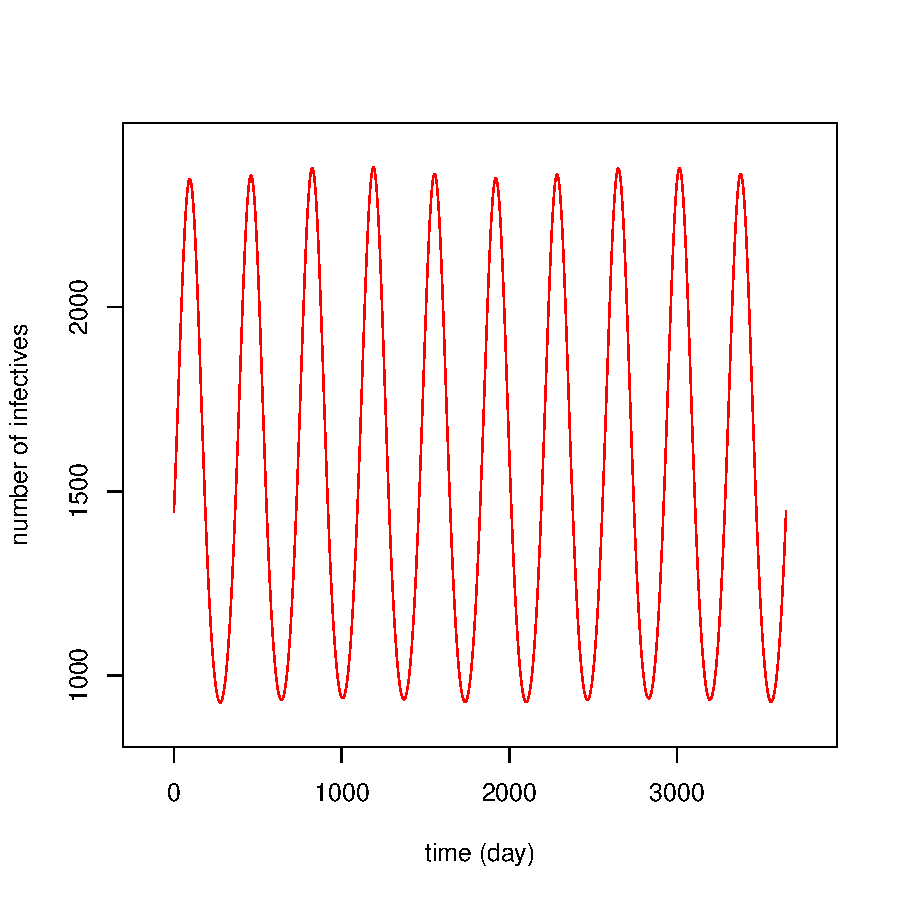
\includegraphics{dizzysNewInfec-001}

Now, we want to continue or to redo this simulation with other values of parameter, we can do it by exploiting the 'globSEIRSimulNewInfec' function in the package.
\begin{Schunk}
\begin{Sinput}
> newobj<- globSEIRSimulNewInfec(obj,duration= 20*365,continue=T, append=T,nbCONTACT0=100, nbCONTACT1=0.0, phiPHASE=pi/2)
> plot(newobj,col="blue",ylab="number of infectives", xlab="time (day)") 
\end{Sinput}
\end{Schunk}
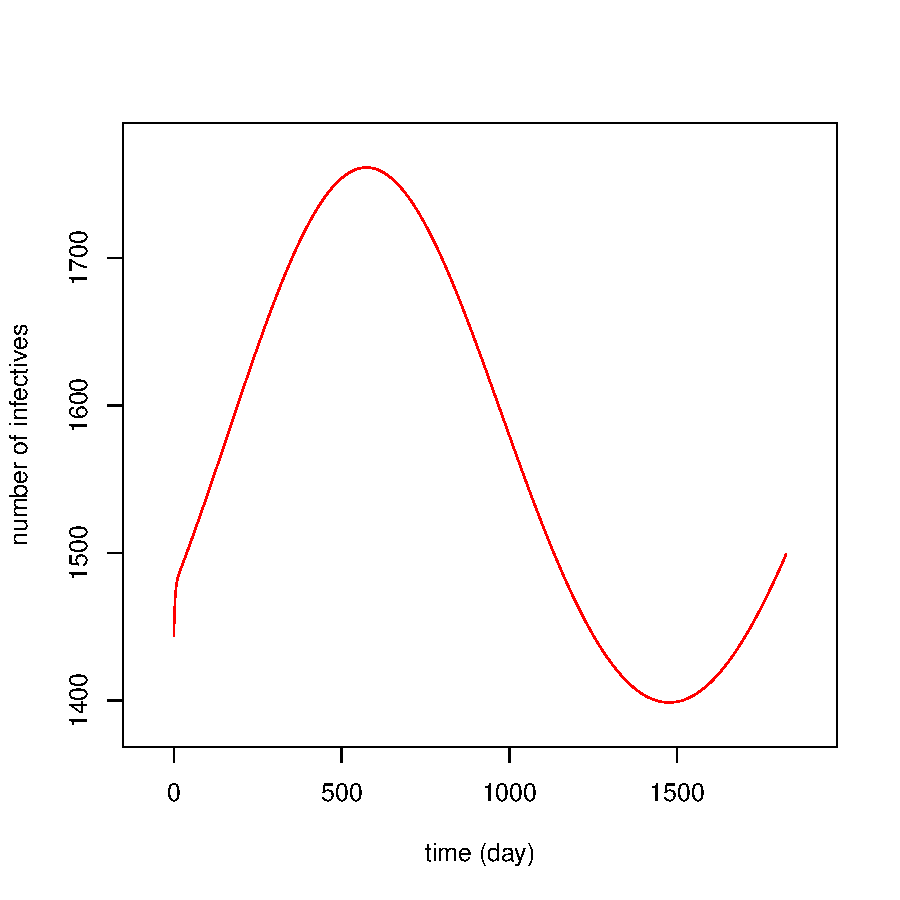
\includegraphics{dizzysNewInfec-002}

\section*{Example 2}

The SEIR stochastic model using Gillespie's algorithm by using the 'seir' function.

1) with one subpopulation:

\begin{Schunk}
\begin{Sinput}
> obj<- globSEIRNewInfec(typeSIMU="stochastic",method="direct",duration=5*365,mu=1/(70*365),sigma=1/8,gamma=1/5,phiPHASE=0,
+ nbVilles=1,S=NULL,E=NULL,I=NULL,R=NULL,N=1e7,nbCONTACT0=100, nbCONTACT1=0.1)
> plot(obj,col="red",ylab="number of infectives", xlab="time (day)") 
\end{Sinput}
\end{Schunk}
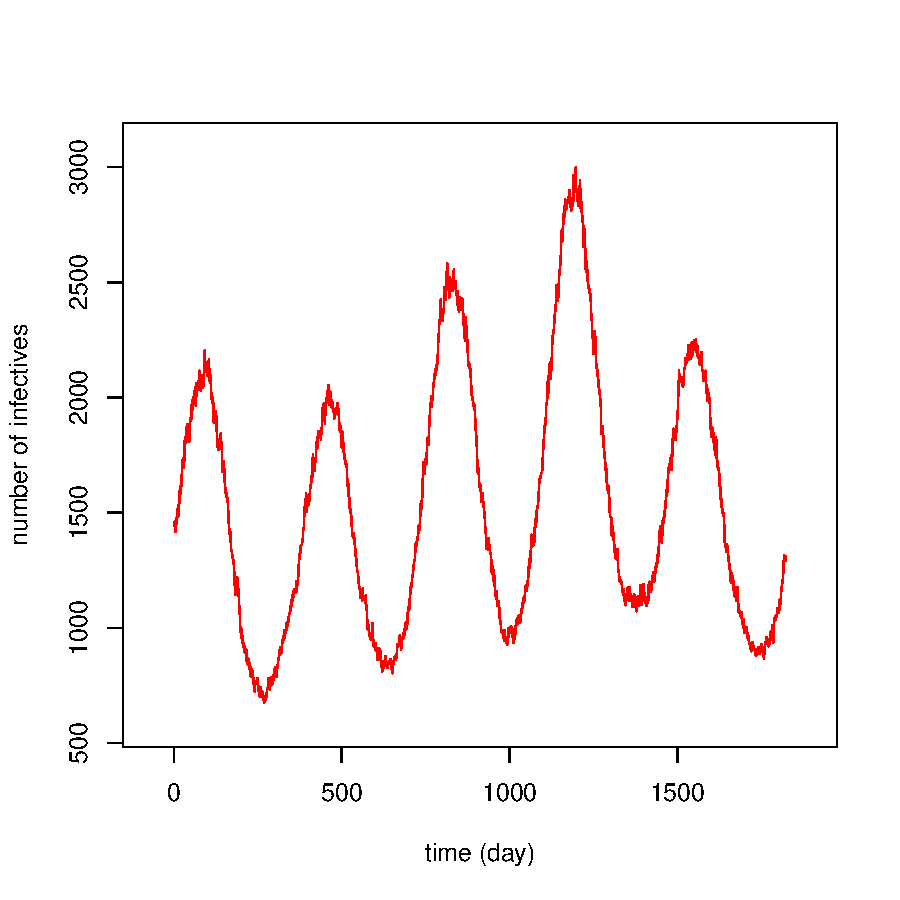
\includegraphics{dizzysNewInfec-003}

2) with three subpopulations and the different number of populations.
\begin{Schunk}
\begin{Sinput}
> obj<- globSEIRNewInfec(typeSIMU="stochastic",duration=5*365,mu=1/(70*365),sigma=1/8,gamma=1/5,nbVilles=3,N=c(1e7,1e6),nbCONTACT0=100, nbCONTACT1=0.1)
> plot(obj,col=c("red","blue"),ylab="number of infectives", xlab="time (day)") 
\end{Sinput}
\end{Schunk}
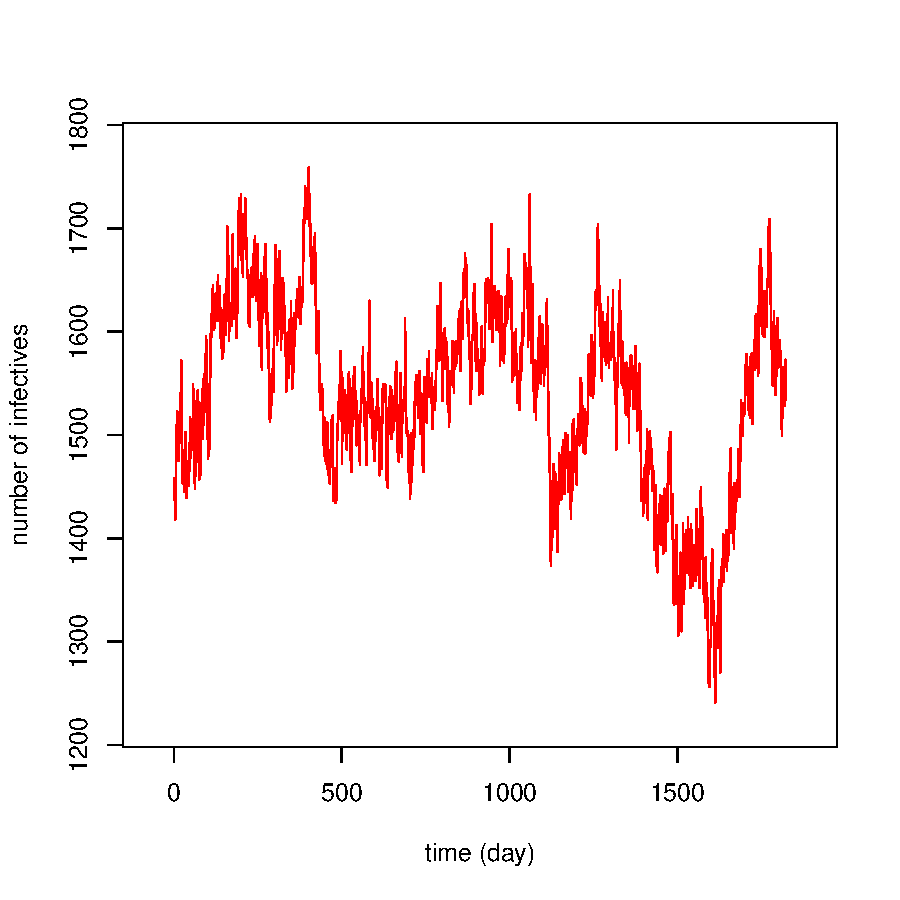
\includegraphics{dizzysNewInfec-004}

3) continue or redo this siluation with other values of parameter, we can do it by exploiting the 'globSEIRSimulNewInfec' function in the package.
\begin{Schunk}
\begin{Sinput}
> newobj<- globSEIRSimulNewInfec(obj,duration= 10*365,typeSIMU="stoch",continue=T,append=T,nbCONTACT0=100,nbCONTACT1=0.0,phiPHASE=pi/2)
> plot(newobj,col=c("red","blue"),ylab="number of infectives",xlab="time (day)")
\end{Sinput}
\end{Schunk}
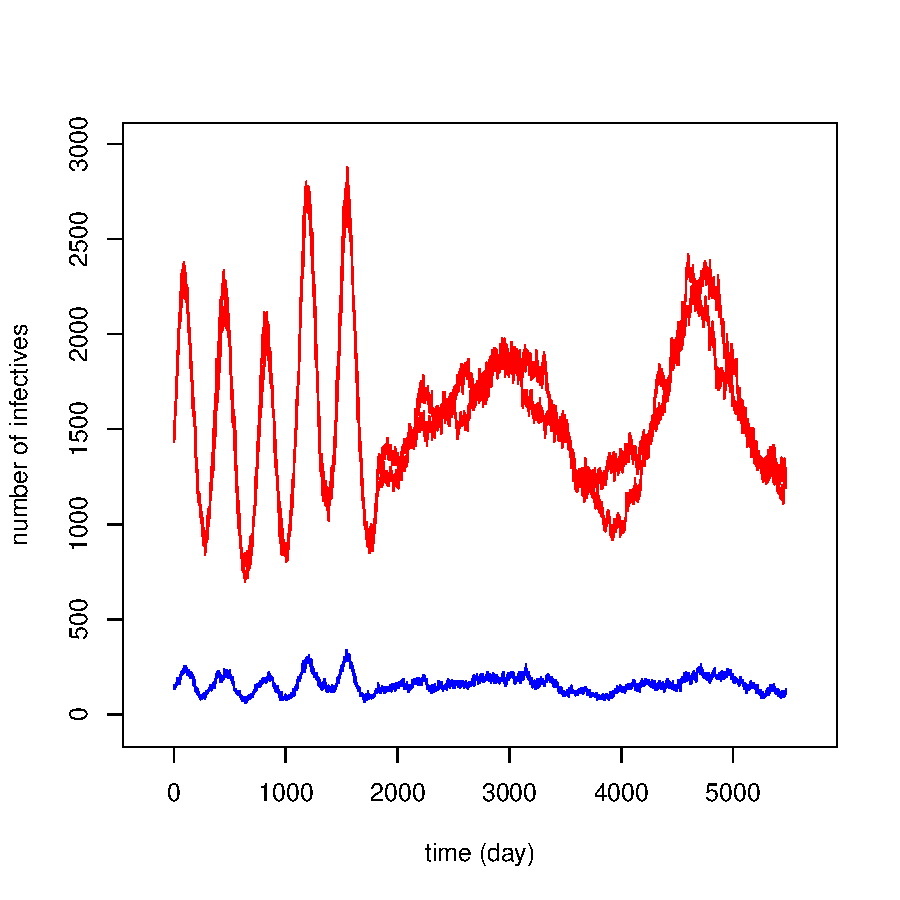
\includegraphics{dizzysNewInfec-005}

\section*{Example 3}

The SEIR stochastic model using "adaptive tau-leaping algorithm" by exploiting the 'globSEIRNewInfec' function. To do this algorithm, we only make the parameter method="adaptivetau" as follows: 
\begin{Schunk}
\begin{Sinput}
> obj<-globSEIRNewInfec(typeSIMU="stochastic",method="adaptivetau",duration=5*365,nbCONTACT0=10000,probVISITER=0.1,probINFECTER=0.1,mu=1/(70*365),sigma=1/8,gamma=1/5,nbVilles=2,N=1e6)
> plot(obj,col=c("red","blue"),ylab="number of infectives", xlab="time (day)") 
\end{Sinput}
\end{Schunk}
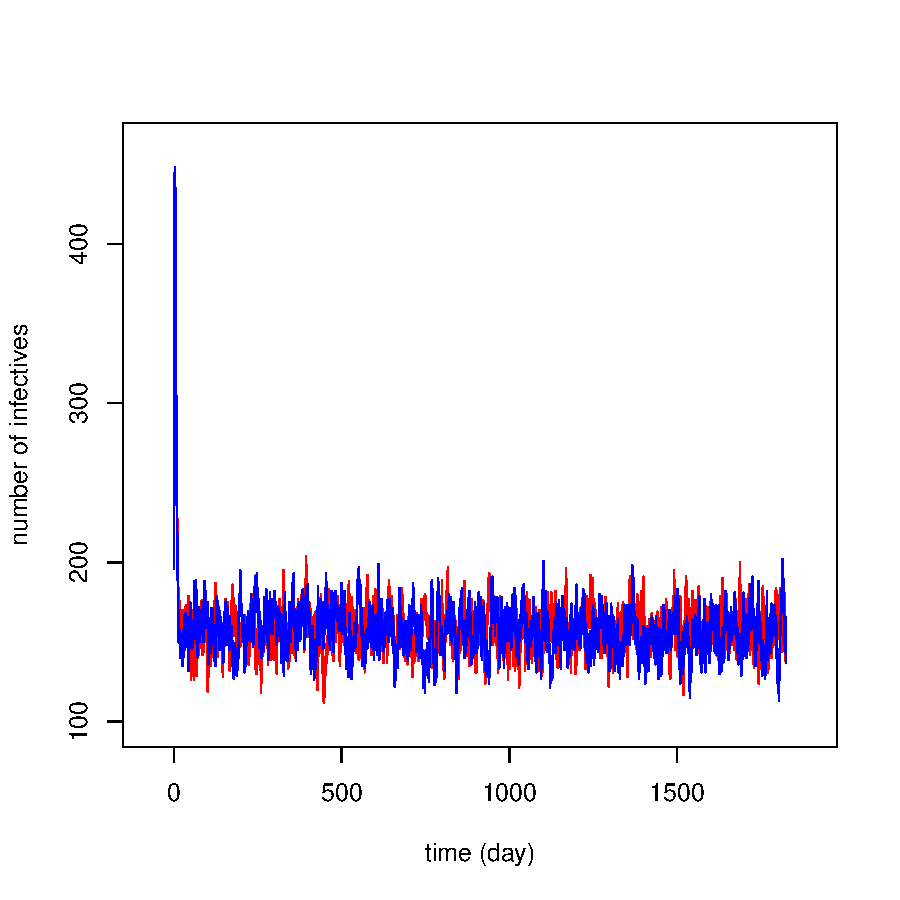
\includegraphics{dizzysNewInfec-006}

We can compare the result of the Gillespie'algorithm with the result of the adaptivetau algorithm:
\begin{Schunk}
\begin{Sinput}
> #obj1 with method="direct"
> obj1<- globSEIRNewInfec(typeSIMU="stochastic",method="direct",
+                         duration=5*365,nbCONTACT0=10000,nbCONTACT1=0.01,
+                         mu=1/(70*365),sigma=1/8,gamma=1/5,nbVilles=1,N=1e6,probVISITER=0.01,probINFECTER=0.1)
> plot(obj1,col="red",ylab="number of infectives", xlab="time (day)") 
> #obj2 with method="adaptivetau"
> obj2<- globSEIRNewInfec(typeSIMU="stochastic",method="adaptivetau",duration=5*365,nbCONTACT0=10000,nbCONTACT1=0.01,
+                         mu=1/(70*365),sigma=1/8,gamma=1/5,nbVilles=1,N=1e6,probVISITER=0.01,probINFECTER=0.1)
> plot(obj2,col="blue",add=T) 
\end{Sinput}
\end{Schunk}
\includegraphics{dizzysNewInfec-007}



\section*{Conclusion} 

Through the above simple examples, the dizzysNewInfec package speeds up simulations and gives exact results on the SIR and SEIR models with the different 
number of subpopulations and the different simulation time. The package successfully implements both an exact solution and an approximate solution. 
Moreover, this hybrid R and C++ implementation pointed out that simulations in this package are faster than any pure R implementation as in the GillespieSSA package. 


\section*{Acknowledgment } 

This package is based on work supported by the Institute for Research and Development at Paris in France and by Professor Jean-Daniel 
Zucker and Marc Choisy. 


\newpage{}
\section*{Appendix} 
\textbf{Goal :} \\
\textbf{Probabilistic derivation of multi-population epidemic model\\
 with $\beta_{ijk}=-\kappa_{j}\log(1-c_{ik})$}
 
\begin{definition}
During the small time interval $\delta t$, each native individual of the city $i$ visits \textbf{a single} city $j$ (with probability $\rho_{ij}$) and will meet \textbf{in average} $\kappa_{j}$ individuals that come from all cities.
\end{definition}

\subsection*{Notation}
\textbf{Notation :}
Here, we present list of sets and events describing the state of the system at time $t$ : 
\begin{itemize}
\item $C_{i}$ is the set of all individuals born in subpopulation $i$. 
\item $V_{i,t}$ is the set of all individuals physically located in subpopulation $i$ from time $t$ to time $t+\delta t$. This includes foreigners traveling in subpopulation $i$ at time $t$, and all natives from subpopulation $i$ which are not traveling abroad at time $t$. 
\item $S_{t},E_{t},I_{t},R_{t}$ are the sets of all individuals respectively susceptible, exposed, infected and recovered at time $t$. Note that these set include individuals from all subpopulations. \item $S_{i,t},E_{i,t},I_{i,t},R_{i,t}$ are the same sets, restricted to natives of subpopulation $i$. So formally, $S_{i,t}=S_{t}\cap C_{i}$, $E_{i,t}=E_{t}\cap C_{i}$, $I_{i,t}=I_{t}\cap C_{i}$, and $R_{i,t}=R_{t}\cap C_{i}$. 
\item $Transmit(y,x)$ is an event indicating that individual $x$ gets
infected by individual $y$ which was already infected \item $c_{i,k}$ is the probability that a susceptible individual native from $i$ being in contact with another infected individual native from $k$ gets infected. 
\item $\kappa_{j}$ is the average number of contacts per unit of time a susceptible will have when visiting city $j$. 
\item $\xi_{jk}$ refers to the probability that an individual $y$ meeting $x$ in $C_{j}$ comes from $C_{k}$.
\item $\rho_{i,j}$, the probability that an individual from subpopulation $i$ visits subpopulation $j$. Of course, $\sum_{j=1}^{M}\rho_{ij}=1$.\end{itemize}

Note that :
The coefficient $\kappa$ should also depend on $i$, because an individual native from city $i$ meets more people in his own city than abroad ($\kappa_{i,i}>\kappa_{i,j}$). 

\subsection*{The background}
\textbf{Let us write a probabilistic formulation of $\frac{dE_{i}}{dt}$:}
One general question is always posed "how does the population of exposed individuals of subpopulation $i$ evolve?". For the sake of simplicity, in the process of transmission of the SEIR model, we focus on the incidence and we assume for now that the latent period and the recovery rate, respectively $\mu=\sigma=0$. Thus, we write a probabilistic formulation of $\frac{dE_{i}}{dt}$. Assuming the time is discrete, we have $\frac{dE_{i}}{dt}\approx\mathbb{E}\left[E_{i,t+1}\setminus E_{i,t}\right]$.
Then,
\begin{eqnarray*}
\mathbb{E}\left[E_{i,t+1}\setminus E_{i,t}\right] & = & \mathbb{E}\left[E_{i,t+1}\cap S_{i,t}\right]\\
 & = & \sum_{x\in C_{i}}Pr\left[x\in E_{t+1}\wedge x\in S_{t}\right]\\
 & = & \sum_{x\in C_{i}}Pr\left[x\in S_{t}\right]*Pr\left[x\in E_{t+1}\mid x\in S_{t}\right]\\
 & = & Pr_{x\sim\mathcal{X}_{i}}\left[x\in E_{t+1}\mid x\in S_{t}\right]*\sum_{x\in C_{i}}Pr\left[x\in S_{t}\right]\\
 & = & |S_{i,t}|\times Pr_{x\sim\mathcal{X}_{i}}\left[x\in E_{t+1}\mid x\in S_{t}\right]
\end{eqnarray*}

Assume there are $M$ cities. An individual $x$ of the subpopulation $i$ may be visiting another subpopulation, or staying in its own
subpopulation. Applying the law of total probabilities, we get: 
\begin{eqnarray*}
Pr_{x\sim\mathcal{X}_{i}}\left[x\in E_{t+dt}\mid x\in S_{t}\right] & = & \sum_{j=1}^{M}Pr_{x\sim\mathcal{X}_{i}}\left[x\in E_{t+dt}\wedge x\in V_{j,t}\mid x\in S_{t}\right]\\
 & = & \sum_{j=1}^{M}Pr_{x\sim\mathcal{X}_{i}}\left[x\in E_{t+dt}\mid x\in S_{t}\wedge x\in V_{j,t}\right].Pr_{x\sim\mathcal{X}_{i}}\left[x\in V_{j,t}\right]\\
 &  & \sum_{j=1}^{M}Pr_{x\sim\mathcal{X}_{i}}\left[x\in E_{t+dt}\mid x\in S_{t}\wedge x\in V_{j,t}\right]\times\rho_{ij}
\end{eqnarray*}

Where $\rho_{i,j}=Pr_{x\sim\mathcal{X}_{i}}\left[x\in V_{j,t}\right]$, the probability that an individual from subpopulation $i$ visits
subpopulation $j$. Of course, $\sum_{j=1}^{M}\rho_{ij}=1$.

\subsubsection*{Study of case where agent $x$ native from subpopulation $i$ visits subpopulation $j$}
Here, we look at the probability that a susceptible $x\sim\mathcal{X}_{i}$ visiting $j$ gets infected or not after $\delta t$ time steps. Let $\mathcal{Y}$ be the uniform distribution over $V_{j,t}$. The correct mathematical approach for this would be to assume that for each subpopulation $k$, the number of people native from $k$ that we meet during $\delta t$
follows a Poisson process. So both the number of people we meet and the number of infected people we meet during $\delta t$ should be random variables.

In the approach described in [KeelingRohani2008], the authors did not do this. They assumed that both the number of people we meet and the number of infected people we meet \emph{are fixed} (otherwise the maths they write would have been different). We will call this the old interpretation of the infection force proposed by "Keeling \& Rohani" (for short, OIIF) that we will present it in the following parts. 
 
We introduce an alternative approximation, where we assume that the number $\kappa$ of people we meet during $\delta t$ is \emph{fixed}, but each of these people has \emph{some probability} to be infected. This is an \emph{in-between interpretation}, easier than the Poisson process maths, but better than the OIIF. We will call this the new interpretation of the infection force (for short, NIIF).

\subsubsection*{The new interpretation: NIIF}
\begin{proposition}
Agent $x$ meets \emph{exactly} $\kappa_{j}$ other individuals, and
each of these individuals has a probability $\frac{\left|I_{k,t}\right|}{N_{k}}$
of being infected, where $k$ is its native subpopulation. Let $y_{1}\ldots y_{\kappa_{j}}$ be the individuals that $x$ meets. We get:
\end{proposition}


\begin{eqnarray*}
 &  & Pr_{x\sim\mathcal{X}_{i}}\left[x\in S_{t+\delta t}\mid x\in S_{t}\wedge x\in V_{j,t}\right]\\
 & = & Pr_{x\sim\mathcal{X}_{i},y_{1}\ldots,y_{\kappa_{j}}\sim\mathcal{Y}}\left[\bigwedge_{p=1}^{\kappa_{j}}\neg\left(y_{p}\in I_{t}\wedge Transmit(y_{p},x)\right)\mid x\in S_{t}\wedge x\in V_{j,t}\right]
\end{eqnarray*}


So we have:
\begin{eqnarray*}
 &  & Pr_{x\sim\mathcal{X}_{i}}\left[x\in S_{t+\delta t}\mid x\in S_{t}\wedge x\in V_{j,t}\right]\\
 & = & Pr_{x\sim\mathcal{X}_{i},y\sim\mathcal{Y}}\left[\neg\left(y\in I_{t}\wedge Transmit(y,x)\right)\mid x\in S_{t}\wedge x\in V_{j,t}\right]^{\kappa_{j}\delta t}
\end{eqnarray*}

Moreover, we have:
\begin{itemize}
\item the probability so that a susceptible individual $x$ is infected
by an infected individual $y$ :
\end{itemize}
\begin{eqnarray*}
 &  & Pr_{x\sim\mathcal{X}_{i},y\sim\mathcal{Y}}\left[y\in I_{t}\wedge Transmit(y,x)\mid x\in S_{t}\wedge x\in V_{j,t}\right]\\
 & = & \sum_{k=1}^{M}Pr_{x\sim\mathcal{X}_{i},y\sim\mathcal{Y}}\left[y\in I_{t}\wedge Transmit(y,x)\mid x\in S_{t}\wedge x\in V_{j,t}\wedge y\in C_{k}\right].Pr_{y\sim\mathcal{Y}}\left(y\in C_{k}\right)\\
 & = & \sum_{k=1}^{M}\left\{ Pr_{x\sim\mathcal{X}_{i},y\sim\mathcal{X}_{k}}\left[y\in I_{t}\mid x\in S_{t}\wedge x\in V_{j,t}\right]\right.\\
 &  & \,\,\,\,\,\left.\times Pr_{x\sim\mathcal{X}_{i},y\sim\mathcal{X}_{k}}\left[Transmit(y,x)\mid y\in I_{t}\wedge x\in S_{t}\wedge x\in V_{j,t}\wedge y\in C_{k}\right]\times Pr_{y\sim\mathcal{Y}}\left(y\in C_{k}\right)\right\} \\
 & = & \sum_{k=1}^{M}\left(\frac{\left|I_{k,t}\right|}{N_{k}}\times c_{ik}\times\xi_{jk}\right)
\end{eqnarray*}


$\xi_{jk}=\frac{N_{k}\rho_{kj}}{\sum_{v=1}^{M}N_{v}\rho_{vj}}$ refers to the probability that an individual $y$ meeting $x$ in $C_{j}$ comes from $C_{k}$.
\begin{itemize}
\item hence, the probability so that a susceptible individual $x$ is not
infected by an infected individual $y$ :
\end{itemize}
\[
1-\sum_{k=1}^{M}\left(\frac{\left|I_{k,t}\right|}{N_{k}}\times c_{ik}\times\xi_{jk}\right)
\]

\begin{itemize}
\item thereby, the probability so that a susceptible individual $x$ is not infected after $\kappa_{j}$ contacts per unit time $\delta t$.
\end{itemize}
\[
\left[1-\sum_{k=1}^{M}\left(\frac{\left|I_{k,t}\right|}{N_{k}}\times c_{ik}\times\xi_{jk}\right)\right]^{\kappa_{j}\delta t}
\]

\begin{itemize}
\item thus, the probability so that a susceptible individual $x$ becomes infected after $\kappa_{j}$ contacts per unit time $\delta t$.
\end{itemize}

\begin{eqnarray*}
Pr_{x\sim\mathcal{X}_{i}}\left[x\in E_{t+\delta t}\mid x\in S_{t}\wedge x\in V_{j,t}\right] & = & \left[1-\sum_{k=1}^{M}\left(\frac{\left|I_{k,t}\right|}{N_{k}}\times c_{ik}\times\xi_{jk}\right)\right]^{\kappa_{j}\delta t}
\end{eqnarray*}
We now apply the \emph{log} approximation which consists in approximating
$1-(1-u)^{v}$ by $v\log(1-u)$:

\begin{eqnarray*}
Pr_{x\sim\mathcal{X}_{i}}\left[x\in E_{t+\delta t}\mid x\in S_{t}\wedge x\in V_{j,t}\right] & = & -\kappa_{j}\delta t\log\left[1-\sum_{k=1}^{M}\left(\frac{\left|I_{k,t}\right|}{N_{k}}\times c_{ik}\times\xi_{jk}\right)\right]
\end{eqnarray*}

So, the transmission rate per susceptible individual is as follows:
\[
\frac{dPr_{x\sim\mathcal{X}_{i}}\left[x\in E_{t+dt}\mid x\in S_{t}\wedge x\in V_{j,t}\right]}{dt}\simeq-\kappa_{j}\log\left[1-\sum_{k=1}^{M}\left(\frac{\left|I_{k,t}\right|}{N_{k}}\times c_{ik}\times\xi_{jk}\right)\right]
\]

In fact, we use the parameter $\lambda$ to present this quantity, and it is denoted as the "force of infection" :
x


If there is only one subpopulation $i$, then
\[
\lambda_{i}=\kappa_{j}log(1-\frac{\left|I_{i}\right|}{N_{i}}\times c_{ii})
\]


\subsubsection*{The old Interpretation : OIIF [KeelingRohani2008]}

\begin{proposition}
Agent $x$ meets \emph{exactly} $\kappa_{j}\delta t\xi_{jk}\frac{\left|I_{k,t}\right|}{N_{k}}$
other infected individuals native from subpopulation $k$.
Let $l_{k}=\kappa_{j}\delta t\xi_{jk}\frac{\left|I_{k,t}\right|}{N_{k}}$. 
Let $y_{1}^{k}\ldots y_{l_{k}}^{k}$ be the infected individuals native
from $k$ that our individual $x$ meets between $t$ and $t+\delta t$.
\end{proposition}

We have the probability so that a susceptible individual $x$ is not infected after having seen $l_{k}$ individuals between $t$ and $t+\delta t$:
\begin{eqnarray*}
 &  & Pr_{x\sim\mathcal{X}_{i}}\left[x\in S_{t+\delta t}\mid x\in S_{t}\wedge x\in V_{j,t}\right]\\
 & = & Pr_{x\sim\mathcal{X}_{i}}\left[\bigwedge_{\begin{array}{c}
k=1\ldots M\\
p=1\ldots l_{k}
\end{array}}\neg\left(Transmit(y_{p}^{k},x)\right)\mid x\in S_{t}\wedge x\in V_{j,t}\right]\\
 & = & \prod_{k=1}^{M}Pr_{x\sim\mathcal{X}_{i}}\left[\bigwedge_{p=1\ldots l_{k}}\neg\left(Transmit(y_{p}^{k},x)\right)\mid x\in S_{t}\wedge x\in V_{j,t}\right]\\
 & = & \prod_{k=1}^{M}\left(1-c_{ik}\right)^{\kappa_{j}\delta t\xi_{jk}\frac{\left|I_{k,t}\right|}{N_{k}}}
\end{eqnarray*}


Then, we plug this back into the previous formula, and we get:
\begin{eqnarray*}
Pr_{x\sim\mathcal{X}_{i}}\left[x\in E_{t+\delta t}\mid x\in S_{t}\wedge x\in V_{j,t}\right] & = & 1-\prod_{k=1}^{M}\left(1-c_{ik}\right)^{\kappa_{j}\xi_{jk}\frac{\left|I_{k,t}\right|}{N_{k}}\delta t}
\end{eqnarray*}

The first order approximation of $1-\prod_{k=1}^{M}(1-c_{ik})^{v_{k}}$
is $\sum_{k=1}^{M}-v_{k}\log(1-c_{ik})$. Applying this approximation here, we get:

\begin{eqnarray*}
Pr_{x\sim\mathcal{X}_{i}}\left[x\in E_{t+\delta t}\mid x\in S_{t}\wedge x\in V_{j,t}\right] & \simeq & \delta t\sum_{k=1}^{M}\left(-\kappa_{j}\xi_{jk}\frac{\left|I_{k,t}\right|}{N_{k}}\log\left(1-c_{ik}\right)\right)
\end{eqnarray*}

Define $\beta_{ijk}=-\kappa_{j}\log\left(1-c_{ik}\right)$, let $\delta t$
converge to zero, and we get:
\[
\frac{dPr_{x\sim\mathcal{X}_{i}}\left[x\in E_{t+dt}\mid x\in S_{t}\wedge x\in V_{j,t}\right]}{dt}\simeq\sum_{k=1}^{M}\left(\xi_{jk}\frac{\left|I_{k,t}\right|}{N_{k}}\beta_{ijk}\right)
\]

If there is only one subpopulation $i$, then we fall back to the formula of [KeelingRohani2008]. We have : 
\[ \beta_{i}=-\kappa_{i}\log\left(1-c_{i}\right) \]
\[\frac{d}{dt}\mathbb{E}\left[\left|E_{i,t+dt}-E_{i,t}\right|\right]\simeq-\left|S_{i,t}\right|\left(\frac{\left|I_{i}\right|}{N_{i}}\beta_{i}\right)\]
and the force of infection as follows :
\[ \lambda_{i}=\beta_{i}\frac{\left|I_{i}\right|}{N_{i}}\]


\subsubsection*{Final Formula}
We simply have to plug in the probability $\rho_{ij}$ that $i$ visits $j$. We get, for the new interpretation NIIF:

\[
\frac{d}{dt}\mathbb{E}\left[\left|E_{i,t+dt}-E_{i,t}\right|\right]\simeq-\left|S_{i,t}\right|\sum_{j}\rho_{ij}\kappa_{j}\log\left[1-\sum_{k=1}^{M}\left(\frac{\left|I_{k,t}\right|}{N_{k}}\times c_{ik}\times\xi_{jk}\right)\right]
\]

And for the old interpretation  OIIF [KeelingRohani2008]:

\[\frac{d}{dt}\mathbb{E}\left[\left|E_{i,t+dt}-E_{i,t}\right|\right]\simeq-\left|S_{i,t}\right|\sum_{j}\rho_{ij}\sum_{k=1}^{M}\left(\xi_{jk}\frac{\left|I_{k,t}\right|}{N_{k}}\beta_{ijk}\right)\]

In conclusion, in this package, we use the interpretation NIIF to present the infection force in meta-population. This interpretation shows enough interactions between individuals in the same city, individuals in different cities, and between cities in meta-population. 



\end{document}
